\subsection{CSDP, C Library for Semidefinite Programming}
\subsubsection{Définition}

Un probl\`eme d\'optimisation convexe avec des in\'egalit\'es matricielles lin\'eaires peut \^etre r\'esolu tr\`es efficacement par programmation semi-d\'efinie.Dans cette recherche , le probl\`eme d\'optimisation est r\'esolu avec la biblioth\`eque C CSDP (C Library for semidefinite programming)\cite{Borchers.B:}.CSDP est \'ecrit en $C$ pour l\'efficacit\'e et la portabilit\'e.\\

CSDP comporte \'egalement un certain nombre de caract\'eristiques qui la rendent tr\`es flexible.CSDP peut travailler avec des matrices sym\'etriques g\'en\'erales ou avec des matrices qui ont une structure diagonale de bloc d\'efinie.Cette biblioth\`eque contient \'egalement des routines pour lire et \'ecrire des probl\`emes SDP et des solutions \`a partir de fichiers.Un programme de r\'esolution autonome est inclus pour r\'esoudre les probl\`emes SDP qui ont \'et\'e \'ecrits dans le format sparse SDPA\cite{SDPA}.

\subsubsection{Le probl\`eme SDP}
CSDP résout les problèmes de programmation semi-définie sous forme:

\begin{equation}
\begin{array}{rrcl}
\max  & \mbox{tr}\; (CX) & & \\
      & A(X) & = & b \\
      & X                   & \succeq & 0 \\
\end{array}
\end{equation}

avec $A_{i}= \mbox{tr}(A_{i}X)$ où $X \succeq 0$ signifie que $X$ est semi-défini positif, $C$ et tous $A_{i}$ sont des matrices symétriques de même taille et $b$ est un vecteur de longueur $m$.\\

Le dual de ce SDP est:

\begin{equation}
\begin{array}{rrcl}
\min  & a^{T}y  & & \\
      & A^{T}(y)-C & = & Z \\
      & Z                   & \succeq & 0 \\
\end{array}
\end{equation}
où
\begin{equation}
A^{T}(y)=\sum_{i=1}^{m} y_{i}A_{i}.
\end{equation}

Et les matrices $C$, $X$ et $Z$ sont traitées comme des matrices diagonales.

\subsubsection{SDP en forme standard}
Considérons, par exemple, le programme semi-défini proposé par le professeur Borchers \cite{Borchers.B:}.Soit le PO a suggéré de résoudre le SDP:

\begin{equation}
\begin{array}{rrcl}
\min  & 0 &&  \\ 
&P - A^{T}PA - \varepsilon I & \succeq & 0 \\ 
&P &\succ & 0\\ 
\end{array}
\end{equation}
% * <assale.adje@gmail.com> 2018-07-27T11:56:27.436Z:
% 
% Ou est passée la valeur propre maximale de P?
% 
% ^.

où $\varepsilon$ est une petite constante positive(nous utiliserons $\varepsilon = 0.01$ dans la suite.) comme $A^{T}P A$ est semi-défini positif et que $\varepsilon I$ est défini positif, ces contraintes imposent $P \succ 0$ (En fait, $P \succeq \varepsilon I $, donc la plus petite valeur propre de $P$ sera supérieur ou égal à $\varepsilon $.) \\

La modélisation de paquets (Packages) comme CVX et Yalmip peuvent facilement transformer cette formulation en un SDP qui peut être résolu par une variété de solveurs tels que SDPT3, SeDuMi, CSDP, SDPA,.. etc.Cependant, le PO veut voir comment transformer cela en une forme standard SDP \cite{Borchers.B:}.



\begin{equation}
\begin{array}{rrcl}
\max  & \mbox{tr}\; (CX)  & & \\
     &\mbox{tr}\;(A_{i}X)&=&b_{i}\;\; i=1, 2, \ldots, m \\
      & X       & \succeq & 0 \\
     
\end{array}
\end{equation}

La première étape consiste à introduire une variable lâche $S$ et à écrire le problème comme  
\begin{equation}
\begin{array}{rrcl}
\max  & 0  & & \\
     & P- A^{T} PA - S &=& \varepsilon I \\
      & S       & \succeq & 0 \\
       & P       & \succeq & 0 \\
\end{array}
\end{equation}

 La contrainte $P- A^{T} PA - S = \varepsilon I$ est linéaire dans les éléments de $P$, bien que cela ne soit pas immédiatement évident.L’observation clé est que  

 \begin{equation}
 A^{T}PA=\underset{ j,k } \sum P_{j,k} \; \underset{i,l} \sum A_{j,i}A_{k,l} E_{i,l}
 \end{equation}  
 
 Par la suite 
 
  \begin{equation}
P- A^{T}PA=\underset{ j,k } \sum P_{j,k} \Big( E_{j,k}- \underset{i,l} \sum A_{j,i}A_{k,l} E_{i,l} \Big)
 \end{equation}  
 
 Et enfin 
 
 
   \begin{equation}
P- A^{T}PA-\varepsilon I=\underset{ j,k } \sum P_{j,k} \underbrace{\Big( E_{j,k}- \underset{i,l} \sum A_{j,i}A_{k,l} E_{i,l} \Big)}_{A_{i}} -\underbrace{\varepsilon I}_{A_{0}} 
 \end{equation}  
% * <assale.adje@gmail.com> 2018-07-27T11:56:58.620Z:
% 
% Il faut terminer le travail en écrivant explicitement le dual à partir de ce LMI.
% 
% ^.
 
 \subParagraphe{Exemple d'application}
 
 \vspace*{.5cm}
 
 Supposons que le PO a une matrice $A$ de taille $(2\times2)$ 
 
 \begin{equation}
A=\left[
\begin{array}{rrrrrrr}
 A_{1,1} & A_{1,2}    \\ 
 A_{2,1} & A_{2,2}   \\ 
    
\end{array}
\right]
\end{equation}


Et pour trouver une matrice symétrique $P$, nous avons besoin de 3 contraintes d'égalité linéaire pour les éléments (1,1), (1,2), (2,2) de l'égalité matricielle 

 \begin{equation}
 \begin{array}{rrcl}
 
&P_{1,1} \left[ E_{1,1} - \left( A_{1,1} A_{1,1} E_{1,1}+ A_{1,1} A_{1,2} E_{1,2}+A_{2,1} A_{1,1} E_{2,1} +A_{1,2} A_{1,2} E_{2,2}       \right) \right] &=&\varepsilon \\

&P_{1,2} \left[ E_{1,2} - \left( A_{1,1} A_{2,1} E_{1,1}+ A_{1,1} A_{2,2} E_{1,2}+A_{1,2} A_{2,1} E_{2,1} +A_{1,2} A_{2,2} E_{2,2}       \right) \right] &=&\varepsilon \\

&P_{2,2} \left[ E_{2,2} - \left( A_{2,1} A_{2,1} E_{1,1}+A_{2,1} A_{2,2} E_{1,2} +A_{2,2} A_{2,1} E_{2,1} + A_{2,2} A_{2,2} E_{2,2}      \right) \right] &=&\varepsilon \\

\end{array}
 \end{equation}
 
 Ensuite
 
   \begin{equation}
 \begin{array}{rrcl}
 
&E_{1,1} \left[ P_{1,1} \left(1-  A_{1,1} A_{1,1}\right)- P_{1,2} \left(  A_{1,1} A_{2,1}\right) -P_{2,1} \left( A_{2,1} A_{1,1}\right) -P_{2,2} \left(A_{2,1} A_{2,1}\right)       \right]-S_{1,1} &=&\varepsilon \\

&E_{1,2} \left[ P_{1,1} \left( A_{1,1} A_{1,2}\right)+ P_{1,2} \left( 1- A_{1,1} A_{2,2}\right) -P_{2,1} \left( A_{2,1} A_{1,2}\right) -P_{2,2} \left( A_{2,1} A_{2,2}\right)       \right]-S_{1,2} &=&\varepsilon \\


&E_{2,2} \left[ P_{1,1} \left( A_{1,2} A_{1,2}\right)- P_{1,2} \left(  A_{1,2} A_{2,2}\right) -P_{2,1} \left( A_{2,2} A_{2,1}\right) +P_{2,2} \left(1-  A_{2,2} A_{2,2}\right)       \right]-S_{2,2} &=&\varepsilon \\


\end{array}
 \end{equation}
 
 
  Enfin nous intégrons $P$ et $S$ dans une matrice diagonale par bloc 
 
 \begin{equation}
X=\left[
\begin{array}{cc}
P &  0\\
0&  S \\
\end{array}
\right]
\end{equation}

Le problème devient
 
 \begin{equation}
\begin{array}{rrcl}
\max  & \mbox{tr}\; (CX)  & & \\
     &\mbox{tr}\;(A_{1}X)&=& \varepsilon \\
     &\mbox{tr}\;(A_{2}X)&=&\varepsilon \\
     &\mbox{tr}\;(A_{3}X)&=& \varepsilon \\
      & X       & \succeq & 0 \\
     
\end{array}
\end{equation}

où 

\begin{equation}
C=0
\end{equation}

\begin{equation}
A_{1}=\left[
\begin{array}{cccc}
1-  A_{1,1} A_{1,1}  &- A_{1,1} A_{2,1} & 0 & 0 \\
- & -A_{2,1} A_{2,1} & 0 & 0 \\
0    &   0  & -1.0 & 0 \\
0    &   0  &  0   & 0 \\
\end{array}
\right]
\end{equation}


\begin{equation}
A_{2}=\left[
\begin{array}{cccc}
-A_{1,1} A_{1,2}& 1- A_{1,1} A_{2,2} & 0 & 0 \\
- & -A_{2,1} A_{2,2} & 0 & 0 \\
0    &   0  &  0 & -1.0 \\
0    &   0  &  0   & 0 \\
\end{array}
\right]
\end{equation}

\begin{equation}
A_{3}=\left[
\begin{array}{cccc}
-A_{1,2} A_{1,2} & - A_{1,2} A_{2,2} & 0 & 0 \\
- & 1-  A_{2,2} A_{2,2} & 0 & 0 \\
0    &   0  &  0 & 0 \\
0    &   0  &  0  & -1.0 \\
\end{array}
\right]
\end{equation}
Prenons l'exemple d'une matrice carrée
 \begin{equation}
A=\left[
\begin{array}{rrrrrrr}
 0.5 & -0.4    \\ 
 1 & -0.5   \\ 
    
\end{array}
\right]
\end{equation}
Après avoir passer par le calcul (2.12) et d'écrire le résultat obtenu sous forme matrice diagonale par bloc, le problème s'écrit au format SDPA comme suit


\begin{lstlisting}
3
2
2 2
0.01 0.01 0.01
1 1 1 1 0.75
1 1 1 2 -0.5
1 1 2 2 -1.0
1 2 1 1 -1.0
2 1 1 1 0.2
2 1 1 2 1.25
2 1 2 2 0.5
2 2 1 2 -1.0
3 1 1 1 -0.16
3 1 1 2 -0.2
3 1 2 2 +0.75
3 2 2 2 -1.0
\end{lstlisting}

Après la résolution de ce problème en utilisant CSDP, on obtient:
\begin{equation}
P=\left[
\begin{array}{cc}
  P_{1,1}   & P_{1,2}\\
 P_{2,1}   & P_{2,2} \\
\end{array}
\right]
=\left[
\begin{array}{cc}
  40.36   & -9.27\\
 -9.27  & 24.39 \\
\end{array}
\right]
\end{equation}

\begin{equation}
S=\left[
\begin{array}{cc}
   S_{1,1}   &   S_{1,2}  \\
S_{2,1}    &  S_{2,2}  \\
\end{array}
\right]
=\left[
\begin{array}{cc}
15.14  & -1.46\\
-1.46   & 15.54 \\
\end{array}
\right]
\end{equation}


Il est facile de vérifier que $P$ possède toutes les propriétés requises.\\
Il y a une infinité de solutions à ce problème il n’y a aucune raison de s’attendre à ce que tous les solveurs renvoient la même solution.\\
On peut également ajuster la fonction objectif ou ajouter des contraintes supplémentaires pour pousser la solution dans une direction souhaitée. Par exemple, on peut vouloir minimiser la valeur propre maximale de $P$ ou minimiser la somme des valeurs propres de $P$.
% * <assale.adje@gmail.com> 2018-07-27T11:59:14.502Z:
% 
% Il faut dire que d'office SDP minimise la valeur propre maximale
% 
% ^.

 \subsubsection{L'interface CSDP}
 
 
 
 









\begin{itemize}
	\itemperso{Trouver une solution initial}
	
	La bibliothèque CSDP contient une routine qui permet d’allouer tout le stockage requis pour trouver une solution initiale. La séquence d’appel pour cette routine est:
                         $$ initsoln(n,k,C,a,constraints,pX0,py0,pZ0).$$
	\itemperso{Appel de la routine SDP}
	
	 C’est une version facile à appeler de la routine sdp.Il prend en entrée un problème sous la forme $$(n, k, C, a, constraints, constant\_offset)$$ et une solution initiale ($X$, $y$, $Z$), allouer l’espace de stockage ensuite faire l’appel à {\tt sdp()} pour résoudre le problème.La solution est retournée dans $X$, $y$, $Z$, {\tt pobj} , {\tt dobj}, et le code de retour de sdp est retourné comme valeur de retour de  {\tt easy\_sdp} (voir 3.1.5).
	
\end{itemize}


\subsubsection{Lecture et écriture de données}

Fonctions pour lire et écrire des données de programme semi-définies et des solutions au format SDPA.


\begin{itemize}
    \itemperso{Usage}
    
read\_prob(fname,pn,pk,pC,pa,pconstraints,printlevel)\\
write\_prob(fname,n,k,C,a,constraints)\\
read\_sol(fname,n,k,C,pX,py,pZ)\\
write\_sol(fname,n,k,X,y,Z)

    
    
    \itemperso{Arguments}
    \begin{itemize}
        \subitemperso{fname} Le nom du fichier à lire ou à écrire.
        \subitemperso{n, pn} La dimension de $X$.
        \subitemperso{k, pk}  Nombre de contraintes.
        \subitemperso{C, pC} La matrice $C$.
        \subitemperso{a, pa} Le vecteur $a$.
        \subitemperso{X, pX} La solution primal $X$.
        \subitemperso{Z, pZ } La matrice dual $Z$.
        \subitemperso{ y,  py} Le vecteur dual $y$.
        \subitemperso{printlevel} $= 0$ pour aucune sortie, $= 1$ pour la normale
                      sortie,$\succ 1$ pour le débogage.
        \subitemperso{ constraints, pconstraints} Les contraintes. 
                      
                      
                      
        
        
    \end{itemize}
    
    \itemperso{Détails}
    
    Les matrices structurées par blocs doivent être spécifiées comme décrit dans\cite{Borchers.B:}.Les fichiers lus doivent être au format SDPA\cite{SDPA}.Cependant, ces fonctions ne prennent pas en charge les commentaires ou les caractères de regroupement par exemple (les accolades, les parenthèses) dans la spécification des tailles de bloc.
    
    \itemperso{Valeurs}
    
    La routine {\tt read\_prob} alloue tout le stockage requis par le problème d’un coté, de l’autre coté {\tt write\_sol}  renvoie 0 en cas de succès et se termine si elle est incapable d’écrire le fichier de solution. 
    
\end{itemize}

\subParagraphe{Spécificités}
\vskip .5cm
\begin{itemize}
    \itemperso{Arguments}
    \begin{itemize}
    \subitemperso{n}  Ce paramètre donne la dimension des matrices $X$, $C$ et $Z$. 
    \subitemperso{k}  Ce paramètre donne le nombre de contraintes.
    \subitemperso{C} Ce paramètre donne la matrice $C$ et définit implicitement la structure en blocs des matrices diagonales.
    \subitemperso{a} Ce paramètre donne le vecteur de droite $a$.
    \subitemperso{constraints} Ce paramètre spécifie les contraintes de problème.
    \subitemperso{constant offset} Ce scalaire est ajouté aux valeurs des objectifs primal et dual.
    
    \subitemperso{pX} En entrée, ce paramètre donne la solution initiale primal X.
    \subitemperso{py} En entrée, ce paramètre donne la solution initiale dual y.
    \subitemperso{pZ} En entrée, ce paramètre donne la solution initiale dual Z.
     \end{itemize}
    
    
    \itemperso{Valeurs}
    \begin{itemize}
        \subitemperso{pX}  En sortie, ce paramètre donne la solution optimale primal X. 
        \subitemperso{py}  En sortie, ce paramètre donne la solution optimale dual y.
        \subitemperso{pZ} En sortie, ce paramètre donne la solution optimale dual Z.
        \subitemperso{ ppobj} Valeur objective optimale primal.
        \subitemperso{pdobj} Valeur objective optimale dual.
    \end{itemize}
    
    \itemperso{Statut}
    
    Statut de la solution renvoyée\\
    \begin{tabular}{r l} 
  
 0 &{\tt Succès }. Problème résolu à une précision totale.  \\ 
 1 &{\tt Succès}. Le problème est irréalisable primal. \\ 
 2 &{\tt Succès}. Le problème est irréalisable dual. \\ 
 3 &{\tt Succès}. partiel. Solution trouvée mais la précision n’a pas été atteinte. \\ 
 4 &{\tt Échec }. Nombre maximal d’itérations atteint. \\ 
 5 &{\tt Échec }. Coincé à la limite de la faisabilité primal. \\  
 6 &{\tt Échec}. Stuc au bord de l’infaisabilité dual. \\ 
 7 &{\tt  Échec}. Manque de progrès. \\ 
 8 &{\tt Échec}. $X$ ou $Z$ (ou Newton système O) est singulier. \\ 
 9 &{\tt Échec }. Valeurs NaN ou Inf détectées. \\ 
  
\end{tabular}
    
    \itemperso{Entrées du programme final}
    \vskip .5cm
    \begin{lstlisting}[language=C++]
#include <stdlib.h>
#include <stdio.h>

/*
 * Include CSDP declarations so that we'll know the calling interfaces.
 */

#include "../include/declarations.h"

/*
 * The main program.  Setup data structures with the problem data, write
 * the problem out in SDPA sparse format, and then solve the problem.
 */
 int main()
{
  /*
   * The problem and solution data.
   */

  struct blockmatrix C;
  double *b;
  struct constraintmatrix *constraints;

  /*
   * Storage for the initial and final solutions.
   */

  struct blockmatrix X,Z;
  double *y;
  double pobj,dobj;

  /*
   * blockptr will be used to point to blocks in constraint matrices.
   */

  struct sparseblock *blockptr;

  /*
   * A return code for the call to easy_sdp().
   */

  int ret,pn,pk;

  /*
   * Write the problem out in SDPA sparse format.
   */

 read_prob("version_final.dat",&pn,&pk,&C,&b,&constraints,0.0);
 write_prob("version_final.dat-s",4,3,C,b,constraints);

  /*
   * Create an initial solution.  This allocates space for X, y, and Z,
   * and sets initial values.
   */

  initsoln(4,3,C,b,constraints,&X,&y,&Z);

  /*
   * Solve the problem.
   */

  ret=easy_sdp(4,3,C,b,constraints,0.0,&X,&y,&Z,&pobj,&dobj);
  if (ret == 0)
    printf("The objective value is %.7e \n",    (dobj+pobj)/2);
  else
    printf("SDP failed.\n");

  /*
   * Write out the problem solution.
   */

  write_sol("version_final.sol",4,3,X,y,Z);

  /*
   * Free storage allocated for the problem and return.
   */

  free_prob(4,3,C,b,constraints,X,y,Z);
  exit(0);
  
}
\end{lstlisting}

 \newpage
 \itemperso{Sortie du programme final}
 \vskip .4cm
 \begin{figure}[ht]
	\centering
	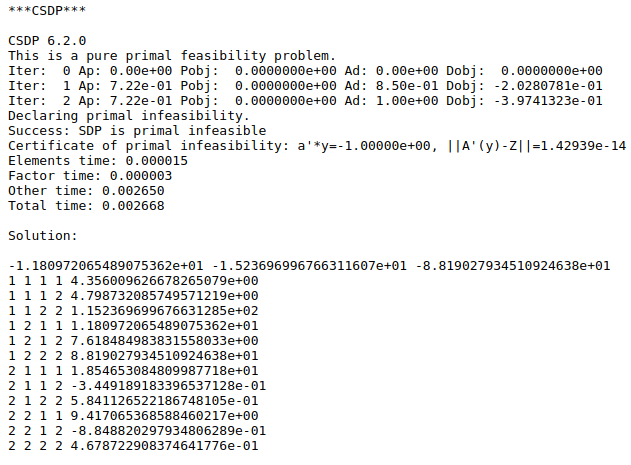
\includegraphics[width=.6\textwidth]{images/output.png}
	\caption{Résultats obtenus après l'appel d'un solveur CSDP}
	\label{fig:CSDP Résult}
\end{figure}

 \end{itemize}
 
 
 
 




